%% 
%% Copyright 2007-2025 Elsevier Ltd
%% 
%% This file is part of the 'Elsarticle Bundle'.
%% ---------------------------------------------
%% 
%% Template article for Elsevier's document class `elsarticle'
%% with numbered style bibliographic references
%% Adapted for Knowledge-Based Systems journal submission
%% 
\documentclass[preprint,12pt]{elsarticle}

%% Use the option review to obtain double line spacing
%% \documentclass[preprint,review,12pt]{elsarticle}

%% Use the options 1p,twocolumn; 3p; 3p,twocolumn; 5p; or 5p,twocolumn
%% for a journal layout:
%% \documentclass[final,1p,times]{elsarticle}
%% \documentclass[final,1p,times,twocolumn]{elsarticle}
%% \documentclass[final,3p,times]{elsarticle}
%% \documentclass[final,3p,times,twocolumn]{elsarticle}
%% \documentclass[final,5p,times]{elsarticle}
%% \documentclass[final,5p,times,twocolumn]{elsarticle}

%% For including figures, graphicx.sty has been loaded in
%% elsarticle.cls. If you prefer to use the old commands
%% please give \usepackage{epsfig}

%% The amssymb package provides various useful mathematical symbols
\usepackage{amssymb}
%% The amsmath package provides various useful equation environments.
\usepackage{amsmath}
%% The amsthm package provides extended theorem environments
%% \usepackage{amsthm}

%% Additional packages for medical imaging paper
\usepackage{algorithmic}
\usepackage{textcomp}
\usepackage{multirow}
\usepackage{url}
\usepackage{subcaption}
\usepackage{microtype}

%% The lineno packages adds line numbers. Start line numbering with
%% \begin{linenumbers}, end it with \end{linenumbers}. Or switch it on
%% for the whole article with \linenumbers.
%% \usepackage{lineno}

\journal{Knowledge-Based Systems}

\begin{document}

\begin{frontmatter}

%% Title, authors and addresses

%% use the tnoteref command within \title for footnotes;
%% use the tnotetext command for theassociated footnote;
%% use the fnref command within \author or \affiliation for footnotes;
%% use the fntext command for theassociated footnote;
%% use the corref command within \author for corresponding author footnotes;
%% use the cortext command for theassociated footnote;
%% use the ead command for the email address,
%% and the form \ead[url] for the home page:

\title{MedDef: An Efficient Self-Attention Model for Adversarial Resilience in Medical Imaging with Unstructured Pruning}

%% use optional labels to link authors explicitly to addresses:
%% \author[label1,label2]{}
%% \affiliation[label1]{organization={},
%%             addressline={},
%%             city={},
%%             postcode={},
%%             state={},
%%             country={}}

\author[a]{E.K. Dongbo}
\author[a]{S. Niu\corref{cor1}}
\author[b]{P. Fero}
\author[b]{P. Bargin}
\author[c]{J.N. Kofa}

\ead{sjniu@hotmail.com}

%% Author affiliations
\affiliation[a]{organization={School of Information Science and Engineering, University of Jinan},
            addressline={}, 
            city={Jinan},
            postcode={250022}, 
            state={Shandong},
            country={P.R. China}}

\affiliation[b]{organization={School of Computer Science \& Technology, Zhejiang Sci-Tech University},
            addressline={}, 
            city={Hangzhou},
            postcode={310018}, 
            state={},
            country={P.R. China}}

\affiliation[c]{organization={College of Informatics, Huazhong Agricultural University},
            addressline={}, 
            city={Wuhan},
            postcode={430070}, 
            state={},
            country={P.R. China}}

\cortext[cor1]{Corresponding author}

%% Abstract (max 250 words)
\begin{abstract}
In an effort to improve diagnostic precision, medical imaging systems are increasingly incorporating artificial intelligence (AI). However, these systems remain susceptible to adversarial attacks, which are subtle, undetectable disruptions intended to trick models into generating inaccurate results. While current methods like adversarial training and input preprocessing provide some partial answers, they frequently reduce diagnostic accuracy by not differentiating between adversarial noise and fine-grained signals that are medically important. We introduce Medical Defense (MedDef), a novel defensive architecture that addresses this challenge by integrating a Defense-Aware Attention Mechanism (DAAM) with unstructured pruning to achieve robust adversarial resilience. DAAM signifies a transition from post-hoc defenses to an integrated approach to robustness, comprising three interrelated components: Adversarial Feature Detection (for noise suppression), Medical Feature Extraction (for domain-specific feature enhancement), and Multi-Scale Feature Analysis (for coordinated multi-resolution defense). These components collaboratively identify and neutralize adversarial noise while amplifying diagnostically critical features. Extensive experiments on Retinal OCT and Chest X-Ray datasets against four common attack methods demonstrate that MedDef achieves exceptional robustness (up to 97.52\% adversarial accuracy) while maintaining high diagnostic accuracy, establishing that security and diagnostic performance can be simultaneously optimized rather than traded off, laying the foundation for clinically viable, adversarially robust medical imaging systems.
\end{abstract}

%%Research highlights
\begin{highlights}
\item Novel Defense-Aware Attention Mechanism (DAAM) integrates adversarial robustness into feature extraction
\item Medical domain-aware defensive strategy preserves diagnostic features while suppressing attacks
\item Unstructured pruning enhances security rather than compromising it in medical imaging
\item Achieves 97.52\% adversarial accuracy with maintained diagnostic performance
\item Comprehensive evaluation on Retinal OCT and Chest X-Ray datasets against multiple attacks
\end{highlights}

%% Keywords (1-7 keywords)
\begin{keyword}
Adversarial Resilience \sep Medical Imaging \sep Defense-Aware Attention Mechanism \sep Unstructured Pruning \sep Robust Model

%% PACS codes here, in the form: \PACS code \sep code
%% MSC codes here, in the form: \MSC code \sep code
%% or \MSC[2008] code \sep code

\end{keyword}

\end{frontmatter}

%% Add \usepackage{lineno} before \begin{document} and uncomment 
%% following line to enable line numbers
%% \linenumbers

%% main text
%%

\section{Introduction}
\label{sec:introduction}

Deep neural networks have revolutionized medical imaging analysis, achieving unprecedented diagnostic accuracy across various conditions~\cite{Mamo24}. While these systems approach or exceed human-level performance in specialized tasks, they remain vulnerable to adversarial attacks; imperceptible perturbations that cause incorrect predictions with potentially serious clinical consequences~\cite{Bortsova21, Kaviani22}.

Current defense strategies fall into several areas, which can be categorically grouped into three: (1) input preprocessing techniques (denoising~\cite{Chiang20}, JPEG compression~\cite{Cheng21}) that neutralize perturbations; (2) model regularization approaches like adversarial training~\cite{Muoka23} that improve robustness; and (3) architectural modifications (defensive distillation~\cite{Qi24}, feature squeezing~\cite{vasan2024}, ensemble methods~\cite{Alzubaidi24}) that detect or mitigate adversarial inputs. 

% Continue with your introduction content...

\section{Related Work}
\label{sec:related_work}

\subsection{Adversarial Defense Techniques in Medical Imaging}
Recent research has increasingly focused on addressing adversarial attacks in medical imaging, which can lead to severe consequences such as misdiagnosis and inaccurate clinical decisions~\cite{Dhamija24}. To solve these issues, a variety of defense tactics have been proposed.

% Continue with related work...

\section{Methodology}
\label{sec:methodology}

This section outline our approach for developing a novel defense-oriented model that synergistically integrates self-attention mechanisms, unstructured pruning, and adversarial training to enhance robustness against adversarial attacks while maintaining high diagnostic accuracy in medical imaging applications.

\subsection{Dataset and Preprocessing}

\subsubsection{Dataset}
Two medical imaging datasets were used: the Retinal OCT (ROCT) dataset (84,484 images across four classes: CNV, DME, Drusen, and Normal) and the Chest X-Ray dataset (5,856 images for binary NORMAL/PNEUMONIA classification).

% Continue with your methodology...

%% Example figure
\begin{figure}[!t]
\centering
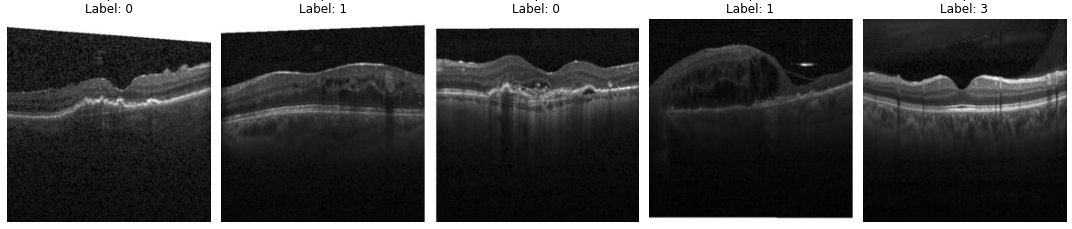
\includegraphics[width=0.9\columnwidth]{fig/fig1_a.png}
\caption{Representative medical imaging samples from both datasets showing retinal cross-sections with varying pathological conditions.}
\label{fig:dataset_samples}
\end{figure}

\section{Experimental Results}
\label{sec:results}

% Your results section

\section{Discussion}
\label{sec:discussion}

% Your discussion section

\section{Conclusion}
\label{sec:conclusion}

% Your conclusions

%% Acknowledgments section
\section*{Acknowledgments}
This research was supported by the National Natural Science Foundation of China (Grant No. 62471202, 62302191), the Natural Science Foundation of Shandong Province (Grant No. ZR2023QF001), Development Program Project of Youth Innovation Team of Institutions of Higher Learning in Shandong Province (Grant No. 2023KJ315), Young Talent of Lifting Engineering for Science and Technology in Shandong (Grant No. SDAST2024QTA014), and the Key Laboratory of Intelligent Computing Technology for Network Environment, Shandong Province, School of Information Science and Engineering, University of Jinan.

%% CRediT authorship contribution statement (required for KBS)
\section*{CRediT authorship contribution statement}
\textbf{E.K. Dongbo:} Conceptualization, Methodology, Software, Validation, Formal analysis, Investigation, Writing – original draft, Writing – review \& editing, Visualization.
\textbf{S. Niu:} Conceptualization, Methodology, Supervision, Project administration, Funding acquisition, Writing – review \& editing.
\textbf{P. Fero:} Methodology, Validation, Investigation, Writing – review \& editing.
\textbf{P. Bargin:} Data curation, Resources, Investigation.
\textbf{J.N. Kofa:} Formal analysis, Investigation, Writing – review \& editing.

%% Declaration of competing interests (required for KBS)
\section*{Declaration of competing interests}
The authors declare that they have no known competing financial interests or personal relationships that could have appeared to influence the work reported in this paper.

%% Data availability statement (required for KBS)
\section*{Data availability}
The datasets used in this study are publicly available: Retinal OCT dataset and Chest X-Ray dataset. Code and additional materials will be made available upon reasonable request.

%% Funding statement (required for KBS)
\section*{Funding}
This work was supported by the National Natural Science Foundation of China [grant numbers 62471202, 62302191]; the Natural Science Foundation of Shandong Province [grant number ZR2023QF001]; Development Program Project of Youth Innovation Team of Institutions of Higher Learning in Shandong Province [grant number 2023KJ315]; Young Talent of Lifting Engineering for Science and Technology in Shandong [grant number SDAST2024QTA014]; and the Key Laboratory of Intelligent Computing Technology for Network Environment, Shandong Province.

%% For citations use: 
%% \cite{<label>} ==> [1]
%% Example citation: See~\cite{lamport94}.

%% If you have bib database file and want bibtex to generate the
%% bibitems, use:
\bibliographystyle{elsarticle-num} 
\bibliography{ref/references}

%% else use the following coding to input the bibitems directly in the
%% TeX file if needed

\end{document}
